\documentclass[12pt,dvipdfmx]{beamer}
\usepackage{graphicx}
\DeclareGraphicsExtensions{.pdf}
\DeclareGraphicsExtensions{.eps}
\graphicspath{{out/tex/svg/}{out/tex/lsvg/}}
\usepackage{listings}
\usepackage{fancybox}
\usepackage{hyperref}
\usepackage{color}

\newcommand{\plusequal}{\mbox{\tt\ += }}
\newcommand{\minusequal}{\mbox{\tt\ -= }}
\newcommand{\divequal}{\mbox{\tt\ /= }}
\newcommand{\plusplus}{\mbox{\tt\ ++ }}

\makeatletter
\newcommand\smallerscriptsize{\@setfontsize\smallerscriptsize\@vipt\@viipt}
\makeatother

%%%%%%%%%%%%%%%%%%%%%%%%%%%
%%% themes
%%%%%%%%%%%%%%%%%%%%%%%%%%%
%\usetheme{Szeged} 
\usetheme{Madrid}

%% no navigation bar
% default boxes Bergen Boadilla Madrid Pittsburgh Rochester
%% tree-like navigation bar
% Antibes JuanLesPins Montpellier
%% toc sidebar
% Berkeley PaloAlto Goettingen Marburg Hannover Berlin Ilmenau Dresden Darmstadt Frankfurt Singapore Szeged
%% Section and Subsection Tables
% Copenhagen Luebeck Malmoe Warsaw

%%%%%%%%%%%%%%%%%%%%%%%%%%%
%%% innerthemes
%%%%%%%%%%%%%%%%%%%%%%%%%%%
% \useinnertheme{circles}       % default circles rectangles rounded inmargin

%%%%%%%%%%%%%%%%%%%%%%%%%%%
%%% outerthemes
%%%%%%%%%%%%%%%%%%%%%%%%%%%
% outertheme
% \useoutertheme{default}       % default infolines miniframes smoothbars sidebar sprit shadow tree smoothtree


%%%%%%%%%%%%%%%%%%%%%%%%%%%
%%% colorthemes
%%%%%%%%%%%%%%%%%%%%%%%%%%%
\usecolortheme{seahorse}
%% special purpose
% default structure sidebartab 
%% complete 
% albatross beetle crane dove fly seagull 
%% inner
% lily orchid rose
%% outer
% whale seahorse dolphin

%%%%%%%%%%%%%%%%%%%%%%%%%%%
%%% fontthemes
%%%%%%%%%%%%%%%%%%%%%%%%%%%
\usefonttheme{serif}  
% default professionalfonts serif structurebold structureitalicserif structuresmallcapsserif

%%%%%%%%%%%%%%%%%%%%%%%%%%%
%%% generally useful beamer settings
%%%%%%%%%%%%%%%%%%%%%%%%%%%
% 
\AtBeginDvi{\special{pdf:tounicode EUC-UCS2}}
% do not show navigation
\setbeamertemplate{navigation symbols}{}
% show page numbers
\setbeamertemplate{footline}[frame number]


%%%%%%%%%%%%%%%%%%%%%%%%%%%
%%% define some colors for convenience
%%%%%%%%%%%%%%%%%%%%%%%%%%%

\newcommand{\mido}[1]{{\color{green!40!black}#1}}
\newcommand{\mura}[1]{{\color{purple}#1}}
\newcommand{\ore}[1]{{\color{orange}#1}}
\newcommand{\ao}[1]{{\color{blue}#1}}
\newcommand{\aka}[1]{{\color{red}#1}}

\setbeamercolor{ex}{bg=cyan!20!white}

%%%%%%%%%%%%%%%%%%%%%%%%%%%
%%% how to typset code
%%%%%%%%%%%%%%%%%%%%%%%%%%%

\lstset{language = C,
numbers = left,
numberstyle = {\tiny \emph},
numbersep = 10pt,
breaklines = true,
breakindent = 40pt,
frame = tlRB,
frameround = ffft,
framesep = 3pt,
rulesep = 1pt,
rulecolor = {\color{blue}},
rulesepcolor = {\color{blue}},
flexiblecolumns = true,
keepspaces = true,
basicstyle = \ttfamily\scriptsize,
identifierstyle = ,
commentstyle = \it\scriptsize,
stringstyle = ,
showstringspaces = false,
tabsize = 4,
escapechar=\@,
}

\title{Understanding GPU performance \\
  {\scriptsize How to get peak FLOPS (GPU version)}}
\institute{}
\author{Kenjiro Taura}
\date{}

\AtBeginSection[] % Do nothing for \section*
{
\begin{frame}
\frametitle{Contents}
\tableofcontents[currentsection,currentsubsection]
\end{frame}
}

\AtBeginSubsection[] % Do nothing for \section*
{
\begin{frame}
\frametitle{Contents}
\tableofcontents[currentsection,currentsubsection]
\end{frame}
}

\begin{document}
\maketitle

%%%%%%%%%%%%%%%%%%%%%%%%%%%%%%%%%% 
\begin{frame}
\frametitle{Contents}
\tableofcontents
\end{frame}


%%%%%%%%%%%%%%%%%%%%%%%%%%%%%%%%%% 
\section{Data Access Performance}
%%%%%%%%%%%%%%%%%%%%%%%%%%%%%%%%%% 
\begin{frame}
  \frametitle{Data access performance}
  \begin{itemize}
  \item data access performance is important in GPU too
  \item 
  \end{itemize}
\end{frame}


\begin{frame}
  \frametitle{Memory organization}

  \begin{itemize}
\item Pascal (P100)

  \begin{center}
    {\small
\begin{tabular}{|c|c|c|c|}\hline
level         & line size & capacity      & associativity \\\hline
L1            & 32B       & 24KB/SM       & ? \\  
L2            & 32B       & 4MB/device    & ? \\
Global Memory &           & 12/16GB       & N/A \\\hline\hline
Shared Memory &           & 64KB ($\ast$) & N/A \\\hline
\end{tabular}}
\end{center}

\item Volta (V100)

  \begin{center}
        {\small
\begin{tabular}{|c|c|c|c|}\hline
level           & line size & capacity              & associativity \\\hline
  L1            & 32B       & 32-128 KB/SM ($\ast$) & ? \\  
  L2            & 32B       & 6MB/device            & ? \\
  Global Memory &           & 16GB                  & N/A \\\hline\hline
  Shared Memory &           & $\leq$96KB ($\ast$)   & N/A \\\hline
\end{tabular}}
\end{center}
\item [] $\ast$ : 128KB is split between L1 and Shared Memory (configurable)
\end{itemize}

source: \url{https://arxiv.org/abs/1804.06826}
\end{frame}

%%%%%%%%%%%%%%%%%%%%%%%%%%%%%%%%%% 
\begin{frame}[fragile]
  \frametitle{Global vs. Shared Memory}
  \begin{itemize}
  \item global memory and L1/L2 cache are the
    ordinary memory that make a hierarchy
    \begin{itemize}
    \item cudaMalloc returns a global memory
    \item accesses to global memory are
      transparently cached into L1/L2 caches
    \end{itemize}
  \item shared memory is an explicitly-managed scratch memory
    \begin{itemize}
    \item latency shorter than L1 (esp. on Pascal)
    \item you explicitly move between global and shared memory
    \item data shared only within a thread block
    \item programming interface is covered shortly
    \end{itemize}
  \end{itemize}
\end{frame}

%%%%%%%%%%%%%%%%%%%%%%%%%%%%%%%%%% 
\begin{frame}[fragile]
  \frametitle{Latency measurement}
  \begin{itemize}
  \item the same pointer chasing experiment as we did on CPU
\begin{lstlisting}
for (@$N$@ times) {
  p = p->next;
}
\end{lstlisting}

\begin{center}
\def\svgwidth{0.6\textwidth}
{\scriptsize \input{out/tex/svg/measure_latency.pdf_tex}}
\end{center}
\end{itemize}
\end{frame}

%%%%%%%%%%%%%%%%%%%%%%%%%%%%%%%%%% 
\begin{frame}[fragile]
  \frametitle{Data size vs. latency}
  \begin{itemize}
  \item even L1 cache hit takes 30 (Volta) - 100 (Pascal) cycles

\begin{center}
%\def\svgwidth{0.6\textwidth}
%{\scriptsize \input{out/tex/data/10mem_gpu/latency}}
out/tex/data/10mem\_gpu/latency
\end{center}
    
  \end{itemize}
\end{frame}


%%%%%%%%%%%%%%%%%%%%%%%%%%%%%%%%%% 
\begin{frame}[fragile]
  \frametitle{Shared memory}

\end{frame}

%%%%%%%%%%%%%%%%%%%%%%%%%%%%%%%%%% 
%%%%%%%%%%%%%%%%%%%%%%%%%%%%%%%%%% 
%%%%%%%%%%%%%%%%%%%%%%%%%%%%%%%%%% 
%%%%%%%%%%%%%%%%%%%%%%%%%%%%%%%%%% 
\end{document}
%%%%%%%%%%%%%%%%%%%%%%%%%%%%%%%%%% 
%%%%%%%%%%%%%%%%%%%%%%%%%%%%%%%%%% 
%%%%%%%%%%%%%%%%%%%%%%%%%%%%%%%%%% 
%%%%%%%%%%%%%%%%%%%%%%%%%%%%%%%%%% 
%%%%%%%%%%%%%%%%%%%%%%%%%%%%%%%%%% 
%%%%%%%%%%%%%%%%%%%%%%%%%%%%%%%%%% 




%%%%%%%%%%%%%%%%%%%%%%%%%%%%%%%%%% 
%%%%%%%%%%%%%%%%%%%%%%%%%%%%%%%%%% 
\section{Recap: the CUDA programming model}
%%%%%%%%%%%%%%%%%%%%%%%%%%%%%%%%%% 
%%%%%%%%%%%%%%%%%%%%%%%%%%%%%%%%%% 

%%%%%%%%%%%%%%%%%%%%%%%%%%%%%%%%%% 
\begin{frame}[fragile]
\frametitle{Recap: the CUDA programming model}
\begin{itemize}
\item you write what a CUDA thread does in
  a device function (or a {\it ``CUDA kernel''})

\begin{lstlisting}
__global__ void f(...) { ... }
\end{lstlisting}
  
\item launch a kernel with many threads

\begin{lstlisting}
f<<<@{\it nb}@,@{\it bs}@>>>(...);
\end{lstlisting}

\end{itemize}
\end{frame}

%%%%%%%%%%%%%%%%%%%%%%%%%%%%%%%%%% 
%%%%%%%%%%%%%%%%%%%%%%%%%%%%%%%%%% 
\begin{frame}
\frametitle{The peak FLOPS of GPUs}
\begin{itemize}
\item \ao{64 SP (32 DP) FMAs per cycle per SM}
  on latest architectures (Pascal and Volta)
\item (except for the much more special-purpose
  half-precision matrix-block multiply operations)

\begin{center}
{\scriptsize
\begin{tabular}{|c|c|c|c|c|c|}\hline
arch                & FMAs   & freq  & SM       & peak   & TDP     \\
                    & /cycle &       &          & GFLOPS &         \\
                    & /SM    &       &          &        &        \\
                    & (SP/DP) & GHz   &         & (SP/DP)  & W       \\\hline
\mura{Pascal {\tiny P100}} & 64/32      & 1.328 & 56 & \mura{9519/4760}  & 300     \\
\mura{Volta {\tiny V100}}  & 64/32      & 1.530 & 80 & \mura{15667/7833} & 300     \\\hline
\end{tabular}}
\end{center}

\item Pascal: 64 $\times$ 2 $\times$ 1.328 $\times$ 56 $=$ 9519
\item Volta: 64 $\times$ 2 $\times$ 1.530 $\times$ 80 $=$ 15667

\end{itemize}
\end{frame}

%%%%%%%%%%%%%%%%%%%%%%%%%%%%%%%%%% 
\begin{frame}
\frametitle{GPU execution hierarchy}
\begin{center}
\only<1>{
\includegraphics[width=0.2\textwidth]{out/pdf/svg/warps_blocks_1.pdf}}%
\only<2-3>{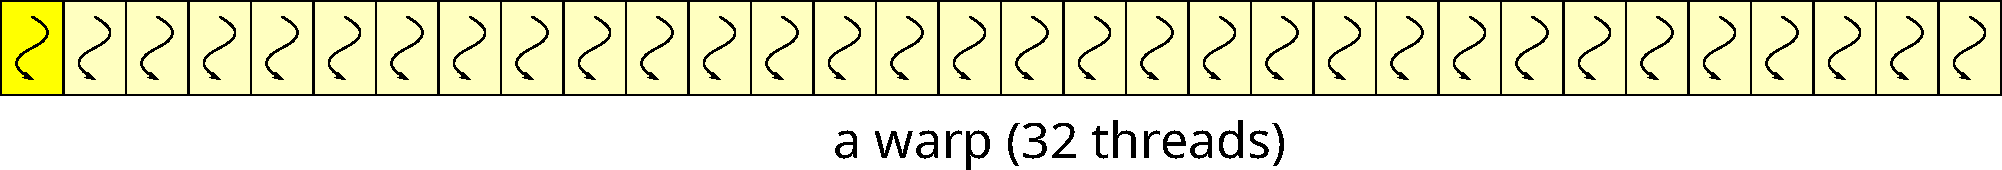
\includegraphics[width=0.7\textwidth]{out/pdf/svg/warps_blocks_2.pdf}}%
\only<4-5>{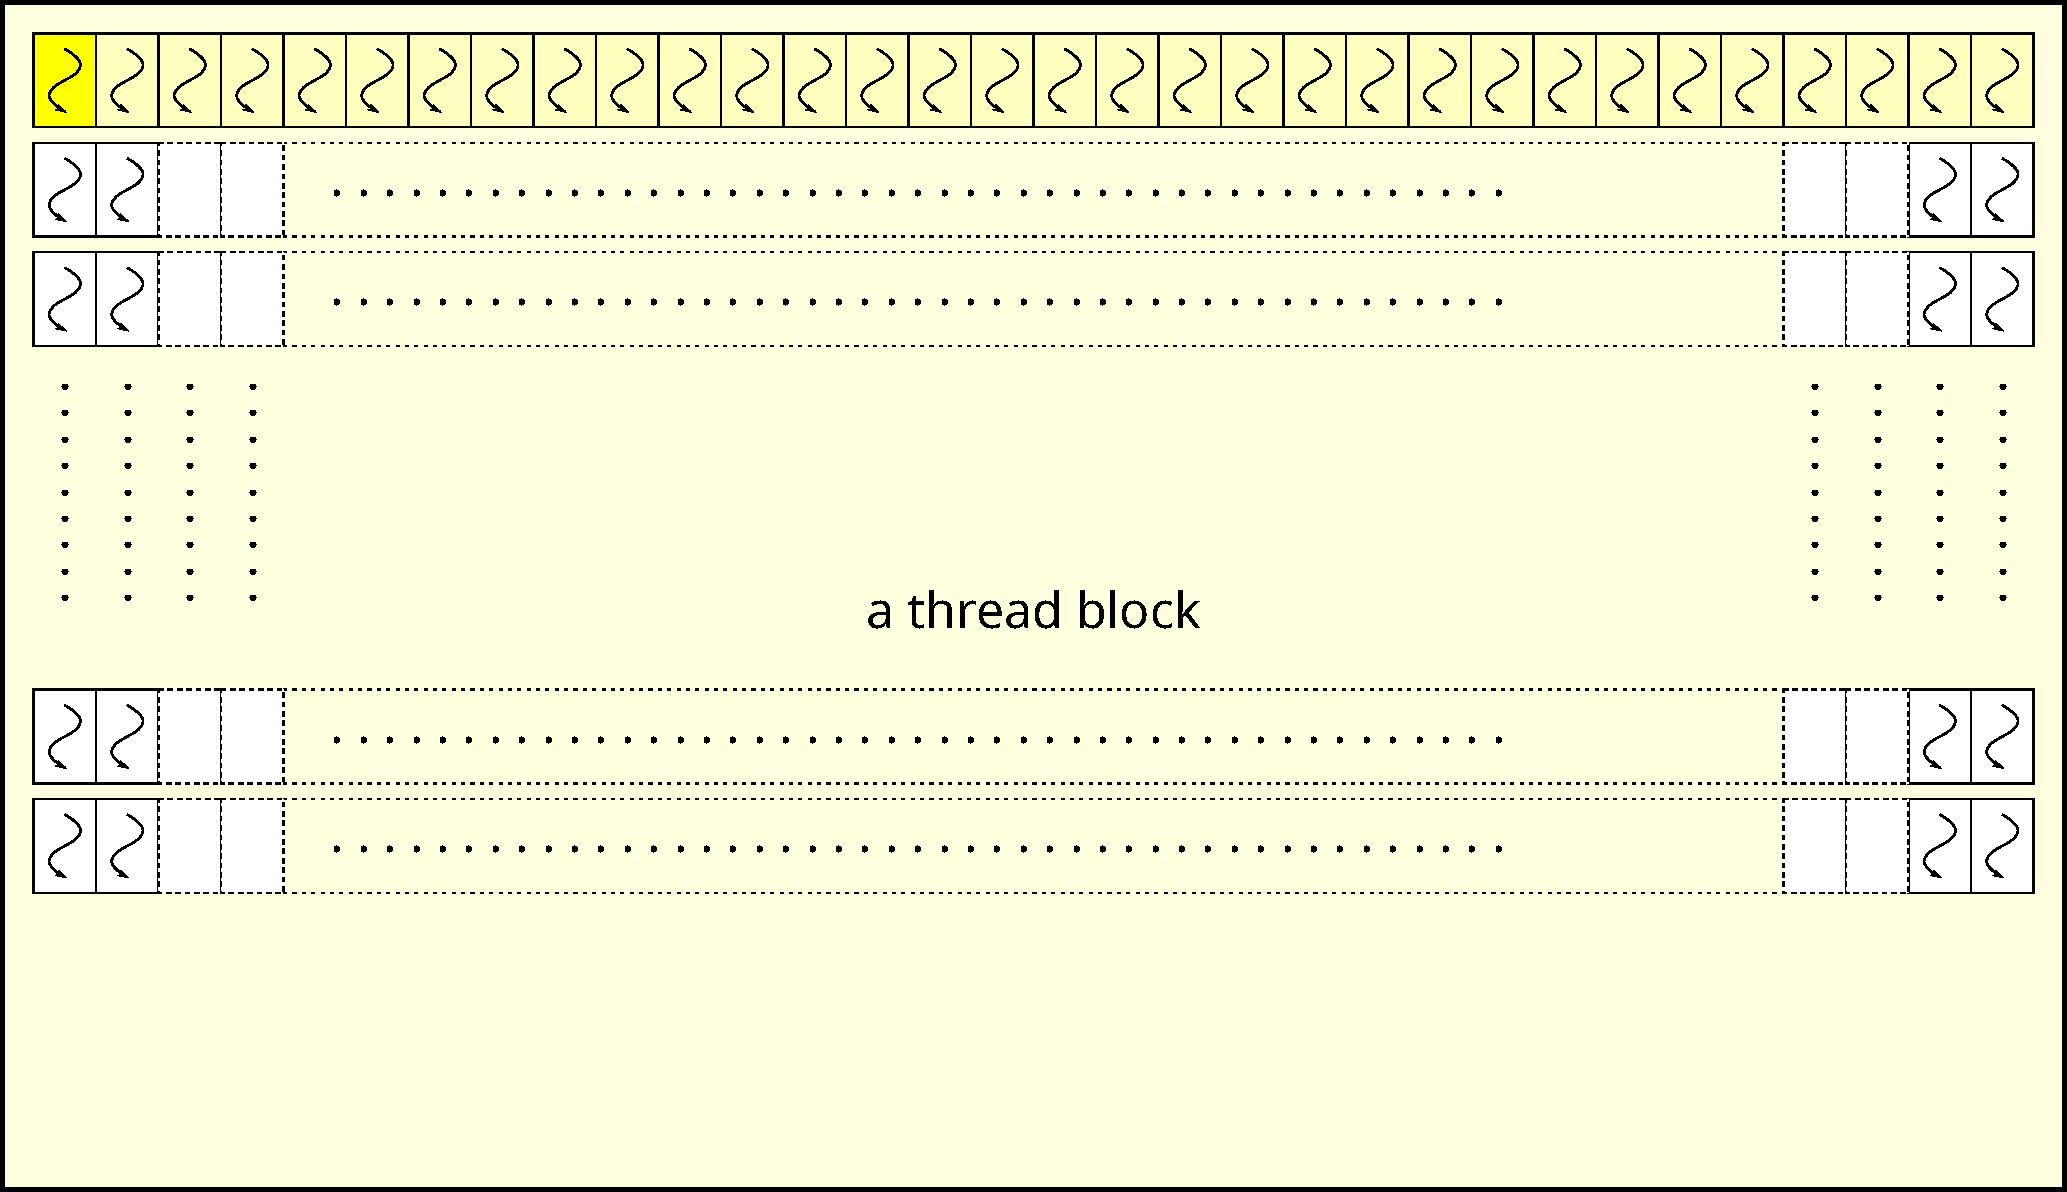
\includegraphics[width=0.7\textwidth]{out/pdf/svg/warps_blocks_3.pdf}}%
\only<6>{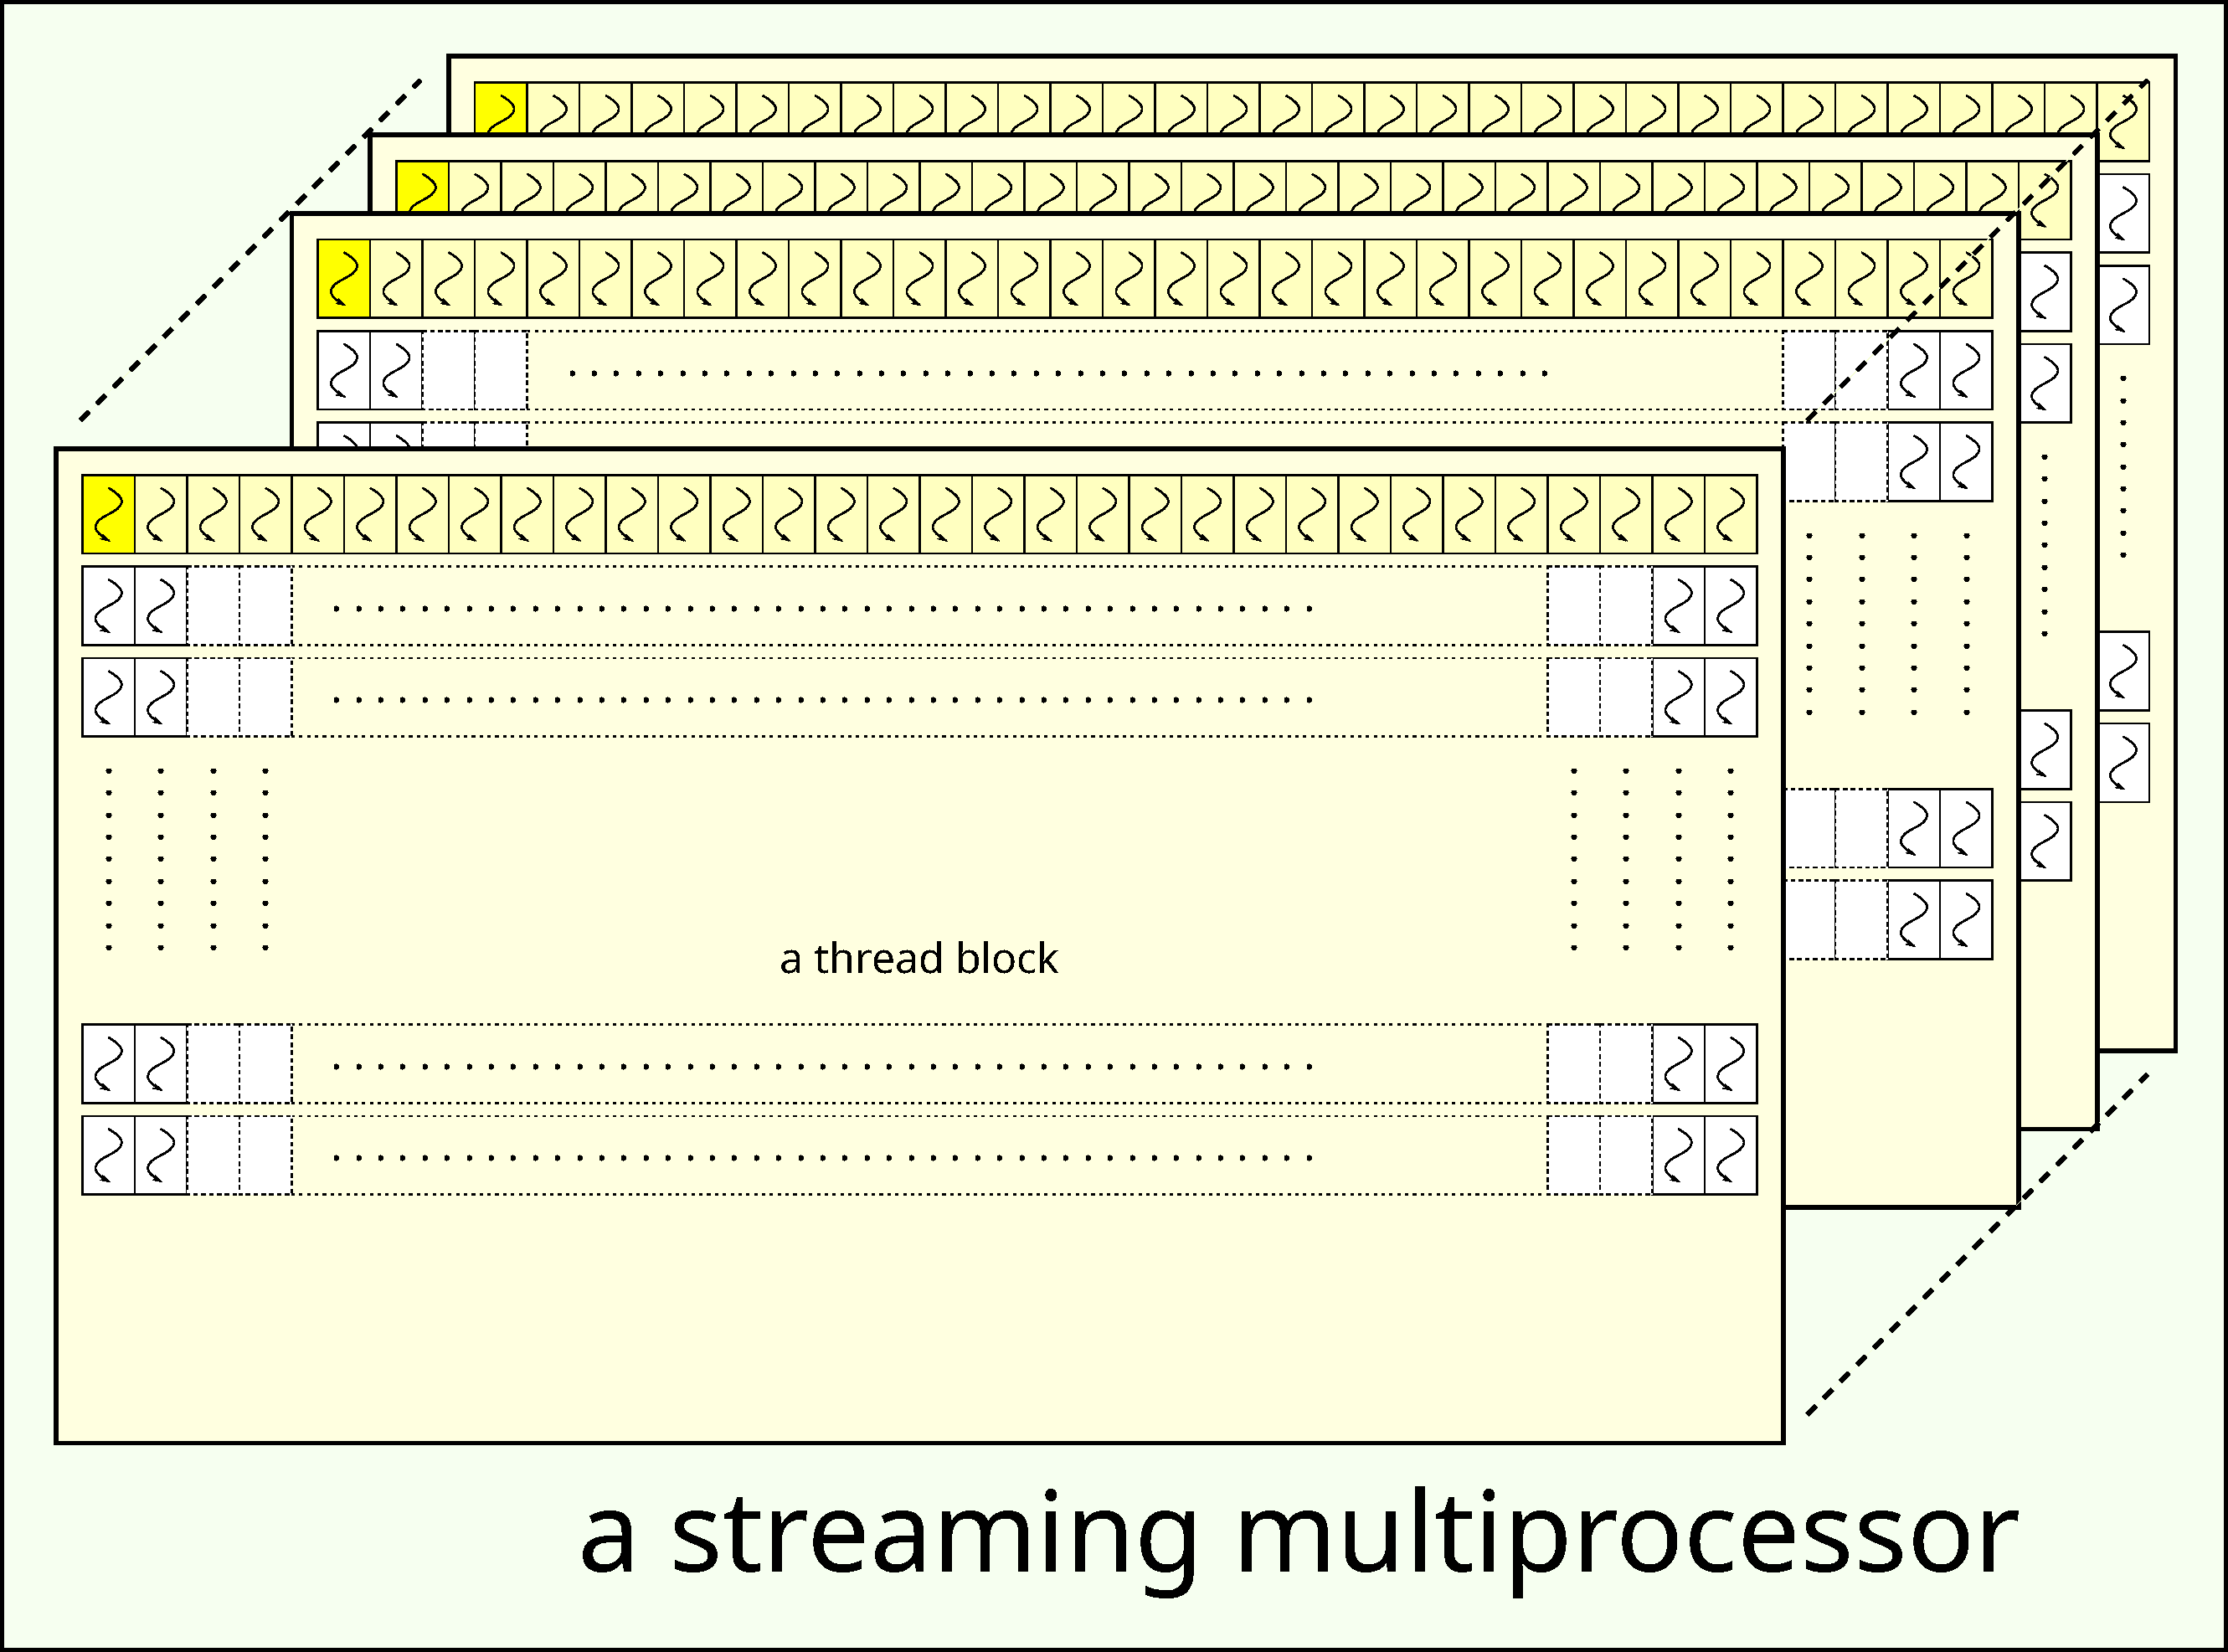
\includegraphics[width=0.7\textwidth]{out/pdf/svg/warps_blocks_4.pdf}}%
\only<7>{\includegraphics[width=0.7\textwidth]{out/pdf/svg/warps_blocks_5.pdf}}%
\end{center}

\only<1>{a kernel function describes a \ao{\it thread}; }

\only<2-3>{32 threads (of consecutive threads IDs) make a \ao{\it warp}; }

\only<3>{threads within a warp execute in a SIMD-like fashion; they execute the same instruction(s) in a cycle; }

\only<4-5>{several warps make a \ao{\it thread block}; }

\only<5>{warps within a block are dispatched to the same \ao{\it Streaming Multiprocessor (SM)}; }

\only<6>{warps in several thread blocks execute in an SM with a fine grain interleaving; }

\only<7>{and there are many SMs in a \ao{\it GPU device}.}

\end{frame}

%%%%%%%%%%%%%%%%%%%%%%%%%%%%%%%%%% 
\begin{frame}
  \frametitle{GPU hierarchy vs. CPU hierarchy}
\begin{center}
\def\svgwidth{\textwidth}
{\scriptsize\input{out/tex/svg/hierarchy_1.pdf_tex}}
\end{center}

\begin{enumerate}
\item<1-> multiple devices (GPU or CPU) on a board
\item<2-> multiple cores (CPU core or SM) in a device
\item<3-> multiple hardware-scheduled
  threads within a core (HWT or thread blocks)
\item<4-> instruction level parallelism within a thread
\item<5-> parallelism within a single instruction (SIMD or warp)
\end{enumerate}
\end{frame}

%%%%%%%%%%%%%%%%%%%%%%%%%%%%%%%%%% 
\begin{frame}
\frametitle{What {\it is} the peak FLOPS (Pascal)?}
\begin{columns}
  \begin{column}{0.6\textwidth}
\begin{itemize}
\item an SM has \ao{2} processing units
\item each processing unit can execute
  1 warp in each cycle and dispatch
  $\leq$ \ao{2} instructions 
  ($\leq$ \ao{1} instruction of the same type)
\item each processing unit has, among others,
  \begin{itemize}
  \item \ao{32 SP (16 DP) FMA} units (each capable of 1 FMA/cycle)
  \item \ao{8 LD/ST} units (each capable of 8 bytes/cycle)
  \end{itemize}

\item $\Rightarrow$
  \ao{peak FLOPS $=$ 2 warps each executing 32 FMAs in a cycle}
\end{itemize}
  \end{column}
  \begin{column}{0.4\textwidth}
\begin{center}
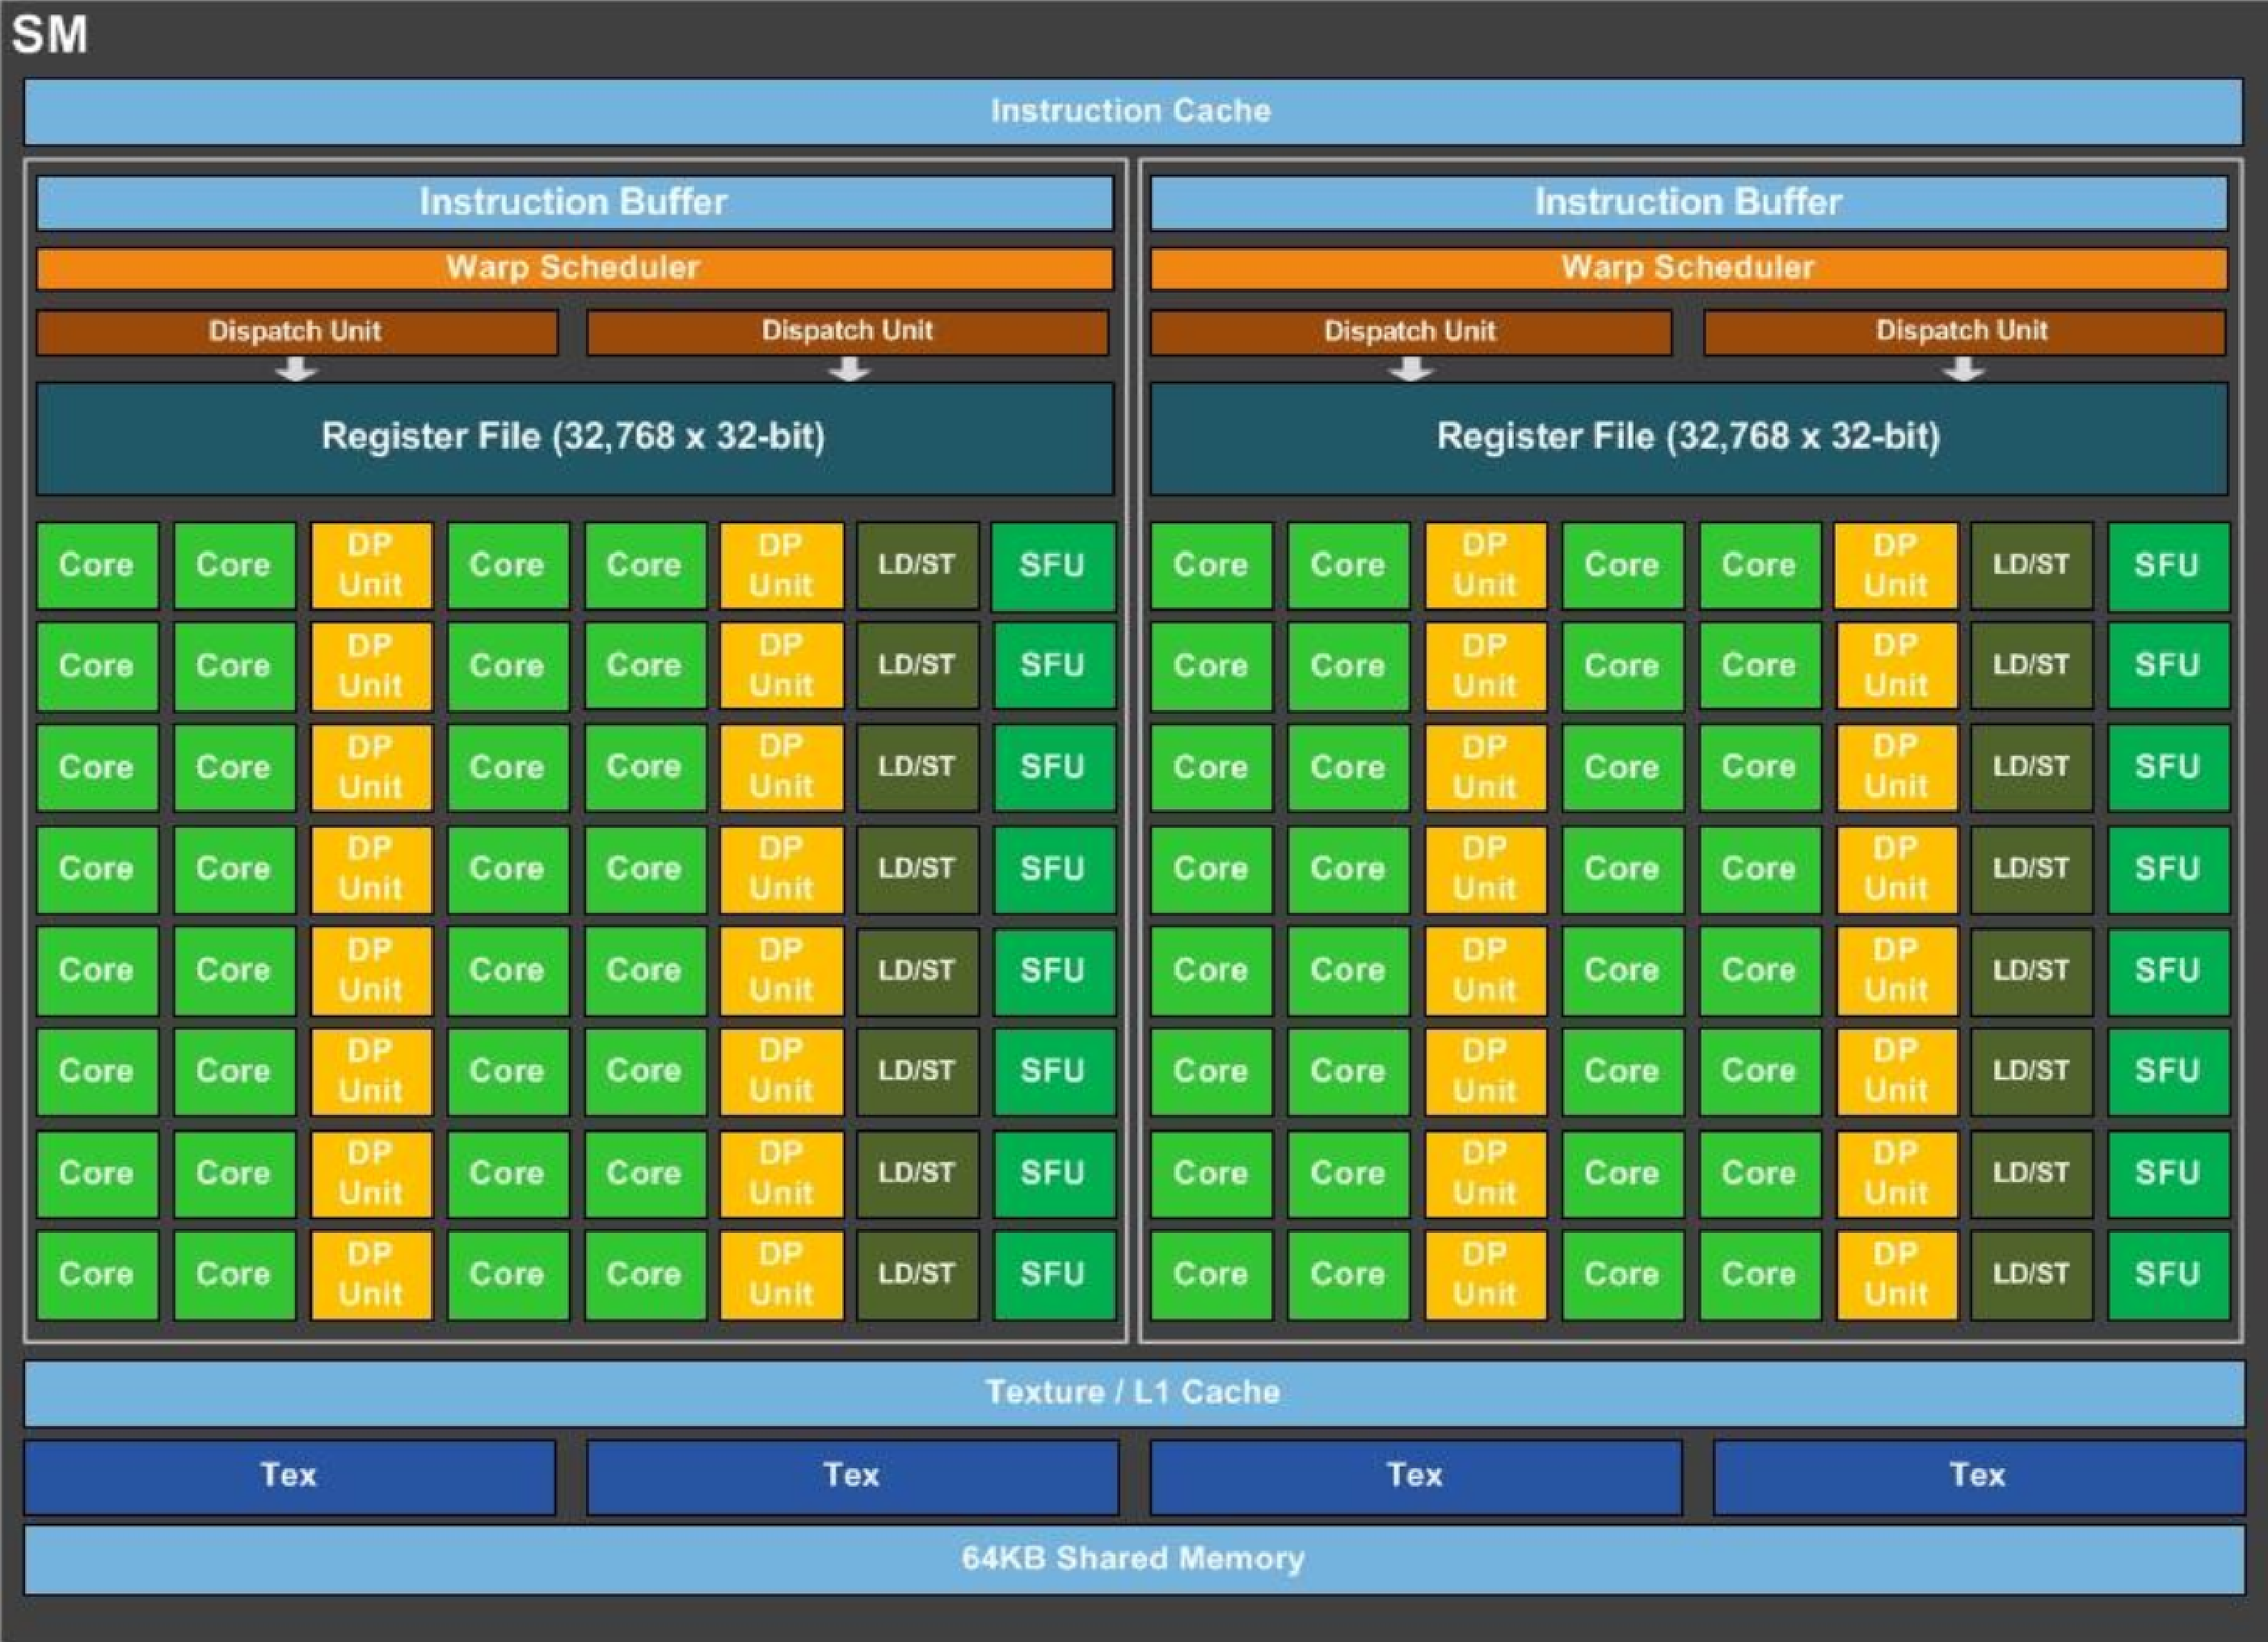
\includegraphics[width=\textwidth]{out/pdf/img/p100sm.pdf}
\end{center}
  \end{column}
\end{columns}

\begin{center}
{\tiny\url{https://images.nvidia.com/content/pdf/tesla/whitepaper/pascal-architecture-whitepaper.pdf}}
\end{center}

\end{frame}

%%%%%%%%%%%%%%%%%%%%%%%%%%%%%%%%%% 
\begin{frame}
\frametitle{What {\it is} the peak FLOPS (Volta)?}
\begin{columns}
  \begin{column}{0.6\textwidth}
\begin{itemize}
\item an SM has \ao{4} processing units
\item each processing unit has, among others
  \begin{itemize}
  \item \ao{16 SP (8 DP) FMA} units (each capable of 1 FMA/cycle)
  \item \ao{8 LD/ST} units (each capable of 8 bytes/cycle)
  \end{itemize}
\item in each cycle, each processing unit can dispatch
  $\leq$ \ao{1} instructions from a warp

\item $\Rightarrow$
  \ao{peak FLOPS $=$ 4 warps each executing 16 FMAs in a cycle}
\end{itemize}
\end{column}
  \begin{column}{0.4\textwidth}

\begin{center}
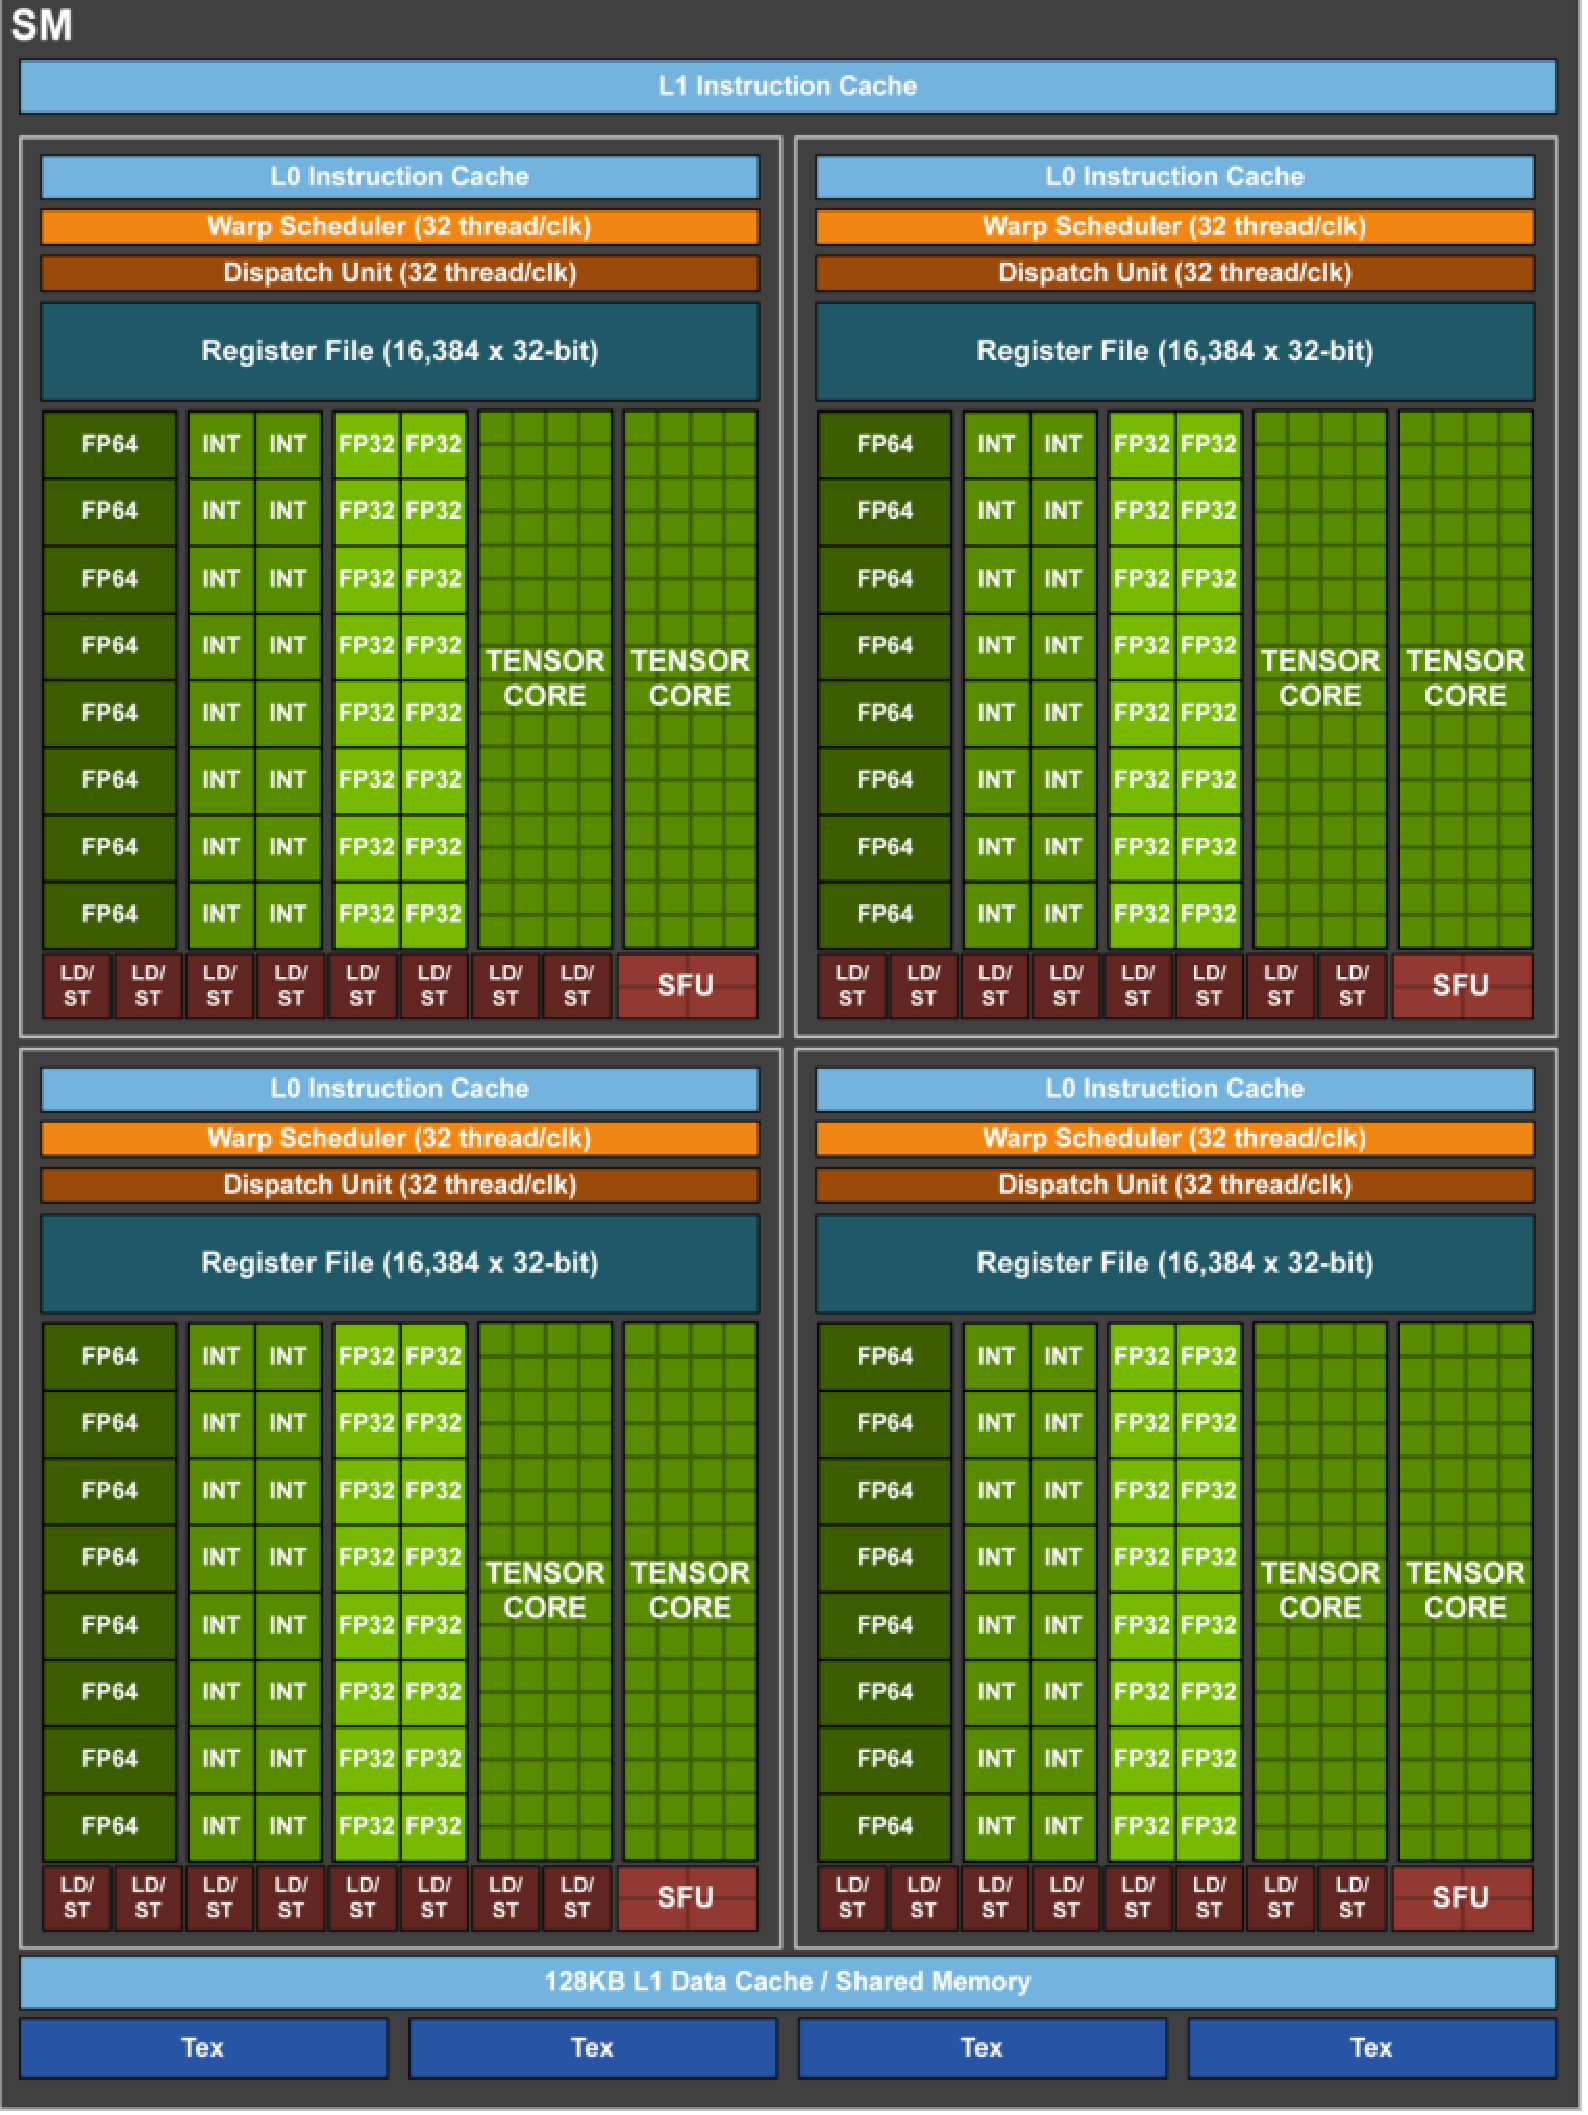
\includegraphics[width=\textwidth]{out/pdf/img/v100sm.pdf}
\end{center}
\end{column}
\end{columns}

\begin{center}
  {\tiny\url{https://images.nvidia.com/content/volta-architecture/pdf/volta-architecture-whitepaper.pdf}}
\end{center}
\end{frame}

%%%%%%%%%%%%%%%%%%%%%%%%%%%%%%%%%% 
%%%%%%%%%%%%%%%%%%%%%%%%%%%%%%%%%% 
\section{An endeavor to nearly peak FLOPS (GPU version)}
%%%%%%%%%%%%%%%%%%%%%%%%%%%%%%%%%% 
%%%%%%%%%%%%%%%%%%%%%%%%%%%%%%%%%% 

%%%%%%%%%%%%%%%%%%%%%%%%%%%%%%%%%% 
\subsection{Latency}
%%%%%%%%%%%%%%%%%%%%%%%%%%%%%%%%%% 
%%%%%%%%%%%%%%%%%%%%%%%%%%%%%%%%%% 
\begin{frame}[fragile]
\frametitle{An endeavor to nearly peak FLOPS}
\begin{itemize}
\item the same ``$x=ax+b$'' iterations that we did on CPU

\begin{lstlisting}
__global__ void axpy_dev(long n, float a, float * X, float b) {
  for (long i = 0; i < n; i++) {
    X[j] = a * X[j] + b;
  }
}
\end{lstlisting}
\end{itemize}
\end{frame}

%%%%%%%%%%%%%%%%%%%%%%%%%%%%%%%%%% 
\begin{frame}[fragile]
\frametitle{A single CUDA thread (Pascal)}
\begin{itemize}
\item run this with a single CUDA thread
\begin{lstlisting}
axpy_dev<<<1,1>>>(n, a, X, b);
\end{lstlisting}
\item compile
\begin{lstlisting}
$ nvcc -o axpy.nvcc -O3 -Xptxas -O3 -x cu --generate-code @\ao{\tt arch=compute\_60,code=sm\_60}@ --compiler-options=-mavx2 axpy.cc
\end{lstlisting} %$
\item run
\begin{lstlisting}
$ srun -p p -t 0:01:00 --gres=gpu:1 ./axpy.nvcc -a cuda
 algo = cuda
    bs = 1 (cuda block size)
    c = 1 (the number of variables to update in the inner loop)
    m = 1 (the number of FP numbers to update)
    n = 1000000 (the number of times to update each variable)
FMAs = 1000000
6690264 clocks, 2126592533 REF clocks, 1250939306 ns
@\ao{\tt 6.690264}@ clocks/iter, 2126.592533 REF clocks/iter, 1250.939306 ns/iter
0.149471 FMAs/clock, 0.000470 FMAs/REF clock, 0.001599 GFLOPS
\end{lstlisting} %$
\end{itemize}
\end{frame}

%%%%%%%%%%%%%%%%%%%%%%%%%%%%%%%%%% 
\begin{frame}[fragile]
\frametitle{A single CUDA thread (Volta)}
\begin{itemize}
\item compile
\begin{lstlisting}
$ make
nvcc -o axpy.nvcc -O3 -Xptxas -O3 -x cu --generate-code @\ao{\tt arch=compute\_70,code=sm\_70}@ --compiler-options=-mavx2 axpy.cc
\end{lstlisting} %$

\item run
\begin{lstlisting}
$ srun -p v -t 0:01:00 --gres=gpu:1 ./axpy.nvcc -a cuda
 algo = cuda
    bs = 1 (cuda block size)
    c = 1 (the number of variables to update in the inner loop)
    m = 1 (the number of FP numbers to update)
    n = 1000000 (the number of times to update each variable)
FMAs = 1000000
4438858 clocks, 4180065444 REF clocks, 1990502355 ns
@\ao{\tt 4.438858}@ clocks/iter, 4180.065444 REF clocks/iter, 1990.502355 ns/iter
0.225283 FMAs/clock, 0.000239 FMAs/REF clock, 0.001005 GFLOPS
\end{lstlisting} %$
\end{itemize}
\end{frame}

%%%%%%%%%%%%%%%%%%%%%%%%%%%%%%%%%% 
\begin{frame}[fragile]
\frametitle{Latencies of common arithmetic}
\begin{itemize}
\item []
\begin{center}
\begin{tabular}{|l|r|r|} \hline
                 & Pascal & Volta \\\hline
integer add      & 6      & 4     \\
integer mul/mad  & 86     & 5     \\
SP add/mul/fma   & \ao{6} & \ao{4}\\
DP add/mul/fma   & 8      & 8     \\\hline
\end{tabular}

{\tiny\url{https://arxiv.org/abs/1804.06826}}
\end{center}
\item measured SP FMA latencies
  \begin{itemize}
  \item Pascal
\begin{lstlisting}
@\ao{\tt 6.690264}@ clocks/iter, @\ldots@
\end{lstlisting}
\item Volta  
\begin{lstlisting}
@\ao{\tt 4.438858}@ clocks/iter, @\ldots@
\end{lstlisting}    
\end{itemize}
\end{itemize}
\end{frame}

%%%%%%%%%%%%%%%%%%%%%%%%%%%%%%%%%% 
\subsection{Looking into Low Level Code}
%%%%%%%%%%%%%%%%%%%%%%%%%%%%%%%%%% 
%%%%%%%%%%%%%%%%%%%%%%%%%%%%%%%%%% 
\begin{frame}
\frametitle{Important options}
\begin{itemize}
\item toolkit documentation:
  \url{https://docs.nvidia.com/cuda/}
\item compiler (nvcc)
  \url{https://docs.nvidia.com/cuda/cuda-compiler-driver-nvcc/index.html}
\item instruction set (PTX)
  \url{https://docs.nvidia.com/cuda/parallel-thread-execution/index.html}
\end{itemize}
\end{frame}

%%%%%%%%%%%%%%%%%%%%%%%%%%%%%%%%%% 
\begin{frame}
\frametitle{Code generation options}
\begin{itemize}
\item there are two kinds of machine code for GPUs
  \begin{itemize}
  \item \ao{PTX (parallel thread execution)} : a portable pseudo assembly
  \item \ao{native code} for each GPU model
  \end{itemize}

\item \ao{\tt --generate-code arch=compute\_{\it nn},code=sm\_{\it nn}}
  instructs nvcc to
  \begin{itemize}
  \item generate PTX assuming a specific architecture
  \item embed the native code for a specific GPU model
  \end{itemize}
  
  \begin{itemize}
  \item \ao{Pascal : {\it nn}$=$60}
  \item \ao{Volta : {\it nn}$=$70}
  \end{itemize}
  
\item you can give {\tt --generate-code} multiple times
  to generate an executable that runs on multiple architectures
    
\item without any {\tt --generate-code} (or similar) options,
  nvcc generates PTX for an old model (sm\_30)
\end{itemize}
\end{frame}

%%%%%%%%%%%%%%%%%%%%%%%%%%%%%%%%%% 
\begin{frame}
\frametitle{Looking into PTX and native code}
\begin{tabular}{|l|l|l|}\hline
{\it xxxx}.ptx      & {\tt nvcc --ptx {\it xxxx}.cu} \\ \hline
{\it xxxx}.fatbin   & {\tt nvcc --fatbin {\it xxxx}.cu}; \\  
native code         & {\tt cuobjdump --dump-sass {\it xxxx}.fatbin > {\it xxxx}.asm} \\
  \hline
\end{tabular}

\begin{itemize}
\item trade offs
\begin{itemize}
\item PTX is easier to deal with; you can embed comments
\item further optimizations apply in the
  PTX $\rightarrow$ native translation, so
  native code may be necessary for precise performance understanding
\end{itemize}
\end{itemize}
\end{frame}


%%%%%%%%%%%%%%%%%%%%%%%%%%%%%%%%%% 
\begin{frame}[fragile]
\frametitle{PTX for axpy}
\begin{itemize}
\item PTX (unrolled four times)
\begin{lstlisting}[escapechar=\!,basicstyle = \ttfamily\tiny],
BB0_11:
  fma.rn.f32  %f15,%f23,%f12,%f13; // f15=f32*f12+f13
  fma.rn.f32  %f16,%f15,%f12,%f13;
  fma.rn.f32  %f17,%f16,%f12,%f13;
  fma.rn.f32  %f23,%f17,%f12,%f13;
  add.s64     %rd36,%rd36,4;
  setp.lt.s64 %p7,%rd36,%rd15;
  @%p7 bra    BB0_11;
\end{lstlisting}
\end{itemize}
\end{frame}

%%%%%%%%%%%%%%%%%%%%%%%%%%%%%%%%%% 
\begin{frame}[fragile]
\frametitle{Native code for axpy}
\begin{itemize}
\item native code for sm\_60 (almost identical for sm\_70)
\begin{lstlisting}[escapechar=\!,basicstyle = \ttfamily\tiny]
/*0328*/ FFMA R9,R9,R11.reuse,c[0x0][0x1a0]; /* 0x5180058006870909 */
/*0330*/ FFMA R9,R9,R11.reuse,c[0x0][0x1a0]; /* 0x5180058006870909 */

  ... 8 FFMA insns ...

/*0390*/ IADD32I R6.CC,R6,0x10;              /* 0x1c10000001070606 */
/*0398*/ FFMA R9,R9,R11,c[0x0][0x1a0];       /* 0x5180058006870909 */
/*03a8*/ IADD.X R7,RZ,R7;                    /* 0x5c1008000077ff07 */
/*03b0*/ FFMA R9,R9,R11.reuse,c[0x0][0x1a0]; /* 0x5180058006870909 */
/*03b8*/ IADD RZ.CC,-R8,R6;                  /* 0x5c128000006708ff */
/*03c8*/ FFMA R9,R9,R11.reuse,c[0x0][0x1a0]; /* 0x5180058006870909 */
/*03d0*/ ISETP.LT.X.AND P1,PT,R7,R10,PT;     /* 0x5b630b8000a7070f */
/*03d8*/ FFMA R9,R9,R11,c[0x0][0x1a0];       /* 0x5180058006870909 */
/*03e8*/ FFMA R9,R9,R11.reuse,c[0x0][0x1a0]; /* 0x5180058006870909 */
/*03f0*/ { FFFMA R9,R9,R11,c[0x0][0x1a0];    /* 0x5180058006870909 */
/*03f8*/   @P1 BRA 0x320;        }           /* 0xe2400ffff201000f */
\end{lstlisting}

\item 16 FFMAs + 4 INTs + 1 branch
\end{itemize}
\end{frame}

%%%%%%%%%%%%%%%%%%%%%%%%%%%%%%%%%% 
\begin{frame}[fragile]
\frametitle{Making sense of the latency results}
\begin{itemize}
\item the reported latency ``6.690264 clocks/iter'' on Pascal suggests
  the above unrolled loop runs in
  \[ 6.690264 \times 16 = 107.044224 = 6 \times 16 + \ao{11} \mbox{ cycles} \]

\item on Volta, it runs in 
  \[ 4.438858 \times 16 = 71.021728  = 4 \times 16 + \ao{7} \mbox{ cycles} \]

\item both are at least close to integers
\item I don't know where these extra 11 / 7 cycles come from \ldots
\end{itemize}
\end{frame}

%%%%%%%%%%%%%%%%%%%%%%%%%%%%%%%%%% 
\begin{frame}[fragile]
\frametitle{Debugging}
\begin{itemize}
\item compile with no optimizations and with debug info
\begin{lstlisting}
$ nvcc @\ao{\tt -O0 -g -G -Xptxas -O0} \ldots
\end{lstlisting} %$

\item use \ao{\tt cuda-gdb}; with slurm, 
  
\begin{lstlisting}
$ srun -p p -t 0:30:00 --gres=gpu:1 @\ao{\tt --pty}@ cuda-gdb @{\it executable}@
\end{lstlisting} %$

\item consider also using \ao{\tt cuda-memcheck}
\end{itemize}
\end{frame}

%%%%%%%%%%%%%%%%%%%%%%%%%%%%%%%%%% 
\subsection{Increasing the Throughput}
%%%%%%%%%%%%%%%%%%%%%%%%%%%%%%%%%% 
%%%%%%%%%%%%%%%%%%%%%%%%%%%%%%%%%% 
\begin{frame}
\frametitle{Increasing the {\it throughput}}
\begin{itemize}
\item the gap to the peak (of a single SM) is enormous
  \begin{itemize}
  \item Pascal: $= 6.690264 \times 64 = 428.17\ldots$
  \item Volta: $= 4.438858 \times 64 = 284.08\ldots$
  \end{itemize}

\item the only way to go beyond this is, of course,
  to increase the parallelism!

\item available tools
  \begin{enumerate}
  \item increase ILP within a thread
    by increasing the number of variables to update
    (just as we did on CPU)
  \item \ao{\it increase the number of threads!}
  \end{enumerate}
\end{itemize}
\end{frame}


%%%%%%%%%%%%%%%%%%%%%%%%%%%%%%%%%% 
\begin{frame}[fragile]
  \frametitle{Increase ILP}
  \begin{itemize}
  \item each thread updates $c$ variables 
\begin{lstlisting}
float X[c];
/* initialize X */
for (long i = 0; i < n; i++)
  for (long j = 0; j < c; j++)
    X[j] = a * X[j] + b;
\end{lstlisting}
\item still launch just a single thread
\begin{lstlisting}
axpy_dev<<<1,1>>>(n, a, X, b);
\end{lstlisting}
\item []
\begin{center}
\def\svgwidth{0.8\textwidth}
{\tiny\input{out/tex/data/06axpy/gpu_single_thread_cuda_c_p.tex}}%
{\tiny\input{out/tex/data/06axpy/gpu_single_thread_cuda_c_v.tex}}
\end{center}
\end{itemize}
\end{frame}

%%%%%%%%%%%%%%%%%%%%%%%%%%%%%%%%%% 
\begin{frame}[fragile]
  \frametitle{Increase the number of threads (in a single SM)}
  \begin{itemize}
  \item this {\it is} the GPU way of increasing parallelism
\begin{lstlisting}
axpy_dev<<<1,@\ao{\it bs}@>>>(n, a, X, b);
\end{lstlisting}
\end{itemize}

\begin{center}
{\tiny\input{out/tex/data/06axpy/gpu_bs_fma_cuda_c_p.tex}}%
{\tiny\input{out/tex/data/06axpy/gpu_bs_fma_cuda_c_v.tex}}
\end{center}

\begin{itemize}
\item the zigzag pattern reflects the number of
  processing units (Pascal: 2, Volta: 4)
\end{itemize}
\end{frame}

%%%%%%%%%%%%%%%%%%%%%%%%%%%%%%%%%% 
\subsection{Programming on GPU and CPU}
%%%%%%%%%%%%%%%%%%%%%%%%%%%%%%%%%% 
%%%%%%%%%%%%%%%%%%%%%%%%%%%%%%%%%% 
\begin{frame}[fragile]
  \frametitle{CUDA {\it unifies} SIMD and thread programming}
  \begin{itemize}
  \item<1-> commonality : both CPU and GPU employ
    a \ao{SIMD-like execution machinery}, for a good peak performance
    with a modest decode/dispatch throughput
    \begin{center}
    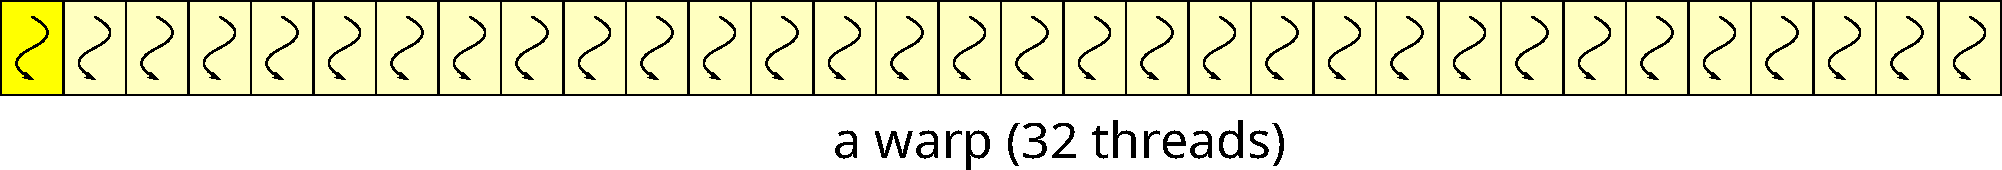
\includegraphics[width=0.7\textwidth]{out/pdf/svg/warps_blocks_2.pdf}
    \end{center}
    
  \item<2-> difference : in CUDA, exploiting SIMD (warp)
    is almost automatic; just increase the number of threads per block
    and GPU executes 32 threads as a warp \ao{(SIMT)}
\begin{lstlisting}
f<<<1,32>>>(x);
\end{lstlisting}
\end{itemize}
\end{frame}

%%%%%%%%%%%%%%%%%%%%%%%%%%%%%%%%%% 
\begin{frame}
  \frametitle{CUDA relieves you from SIMD programming}
  \begin{itemize}
  \item GPU handles many things that hinder vectorization on CPU
    \begin{tabular}{|l|l|}\hline
      issues & how you do it on CPU \\\hline
      branches & predicated execution \\\hline
      loops whose trip counts & predicated execution \\
      vary across threads     &  \\\hline
      non-contiguous data accesses & gather/scatter \\
      atomic update & N/A \\\hline
    \end{tabular}
  \item a great boon to the programmer
  \item note that the performance penalty
    \ao{\it is} still visible on GPUs too
  \end{itemize}
\end{frame}

%%%%%%%%%%%%%%%%%%%%%%%%%%%%%%%%%% 
\begin{frame}[fragile]
  \frametitle{GPU core is {\it highly} multithreaded}
  \begin{itemize}
  \item<1-> commonality : a single thread (warp) performance is often
    limited by \aka{\it latencies}
  \item<2-> commonality : both CPU cores and GPU SMs
    are \ao{\it multithreaded (SMT)}; i.e., each core (SM)
    can simultaneously execute multiple threads (warps),
    switching between them every few cycles

      \begin{columns}
      \begin{column}{0.7\textwidth}
\def\svgwidth{0.9\textwidth}
{\tiny\input{out/tex/svg/hierarchy_1.pdf_tex}}%
\end{column}
\begin{column}{0.3\textwidth}
{\scriptsize\begin{tabular}{|l|r|}\hline
  recent Xeon's & 2 \\
  Xeon Phi      & 4 \\
  Power 9       & 8 \\
  Nvidia GPUs   & \ao{64} \\\hline
\end{tabular}}
\end{column}
\end{columns}
\item<3-> difference : GPU SMs are \ao{\it highly} multithreaded
  \begin{itemize}
  \item each SM supports up to 2048 threads (64 warps)
  \end{itemize}
  \end{itemize}
\end{frame}

%%%%%%%%%%%%%%%%%%%%%%%%%%%%%%%%%% 
\subsection{A Deeper Look at Throughput}
%%%%%%%%%%%%%%%%%%%%%%%%%%%%%%%%%% 
%%%%%%%%%%%%%%%%%%%%%%%%%%%%%%%%%% 
\begin{frame}[fragile]
  \frametitle{Making sense of the gap to the peak (Pascal)}
  \begin{columns}
    \begin{column}{0.5\textwidth}
{\tiny\input{out/tex/data/06axpy/gpu_bs_fma_cuda_c_p.tex}}
    \end{column}
    \begin{column}{0.5\textwidth}
{\scriptsize
\begin{tabular}{|r|r|r|r|} \hline
threads & warps & cycles & FMAs/cycle \\\hline
384 & 12 & 8413085 & 45.64 \\\hline
416 & 13 & 9502041 & 43.78 \\
448 & 14 & 9491826 & 47.19 \\\hline
480 & 15 & 10863789 & 44.18 \\
512 & 16 & 10862553 & 47.13 \\\hline
544 & 17 & 12944833 & 42.02 \\
576 & 18 & 12910888 & 44.61 \\\hline
\end{tabular}}
    \end{column}
  \end{columns}

\begin{itemize}
\item from the latency ($6.690264 \mbox{ cycles/FMA}$),
  we hope that, even with $c = 1$ (each thread updating
  just a single variable), they reach 64 FMAs/cycle with
  \[ 64 \times 6.690264 = 428.17\ldots
    \rightarrow 448 \mbox{ threads (14 warps)} \]
\item the actual peak throughput plateaus at $\approx$ 47 FMAs/sec
\end{itemize}
\end{frame}

%%%%%%%%%%%%%%%%%%%%%%%%%%%%%%%%%% 
\begin{frame}
  \frametitle{Making sense of the gap to the peak (Pascal)}
  \begin{itemize}
  \item Pascal dispatches both SP arithmetic and INT arithmetic
    to the same execution unit (CUDA Core)
  \item \aka{\it overhead of integer instructions are often not negligible on Pascal}

  \item the number of integer instructions is a good predictor
    of the throughput limit
    {\scriptsize
    \begin{tabular}{|c|c|c|l|r|r|}\hline
      $c$ & SP & INT      & FMAs/cycle  & FMAs/cycle  & the thread \\
          & insns & insns & (predicted) & (measured)  & count  \\\hline
      1 & 16 & 4 & $64 \times 16/20 = 51.2$   & $47.19$ & 448 \\
      2 & 32 & 5 & $64 \times 32/37 = 55.35$  & $55.21$ & 512 \\
      3 & 48 & 5 & $64 \times 48/53 = 57.96$  & $57.91$ & 384 \\
      4 & 64 & 5 & $64 \times 64/69 = 59.36$  & $59.33$ & 384 \\
      5 & 20 & 5 & $64 \times 20/25 = 51.2$   & $50.72$ & 448 \\
      6 & 24 & 5 & $64 \times 24/29 = 52.96$  & $52.93$ & 384 \\
      7 & 28 & 5 & $64 \times 28/33 = 54.30$  & $54.23$ & 512 \\
      8 & 32 & 5 & $64 \times 32/37 = 55.35$  & $55.29$ & 384 \\\hline
    \end{tabular}}
  \end{itemize}

\end{frame}

%%%%%%%%%%%%%%%%%%%%%%%%%%%%%%%%%% 
\begin{frame}[fragile]
  \frametitle{Making sense of the zigzag pattern}
  \begin{columns}
    \begin{column}{0.5\textwidth}
  \begin{itemize}
  \item Pascal (2 processing units)
    
{\tiny
\begin{tabular}{|r|r|r|r|} \hline
threads & warps & \ao{cycles} & FMAs/cycle \\\hline
384 & 12 & \ao{8413085} & 45.64 \\\hline
416 & 13 & \ao{9502041} & 43.78 \\
448 & 14 & \ao{9491826} & 47.19 \\\hline
480 & 15 & \ao{10863789} & 44.18 \\
512 & 16 & \ao{10862553} & 47.13 \\\hline
544 & 17 & \ao{12944833} & 42.02 \\
576 & 18 & \ao{12910888} & 44.61 \\\hline
\end{tabular}}
\item Volta (4 processing units)
  
{\tiny
\begin{tabular}{|r|r|r|r|} \hline
threads & warps & \ao{cycles} & FMAs/cycle \\\hline
384 & 12 & \ao{6648872} & 57.75 \\\hline
416 & 13 & \ao{8666550} & 48.00 \\
448 & 14 & \ao{8693014} & 51.53 \\
480 & 15 & \ao{8704994} & 55.14 \\
512 & 16 & \ao{8696415} & 58.87 \\\hline
544 & 17 & \ao{10878118} & 50.00 \\
576 & 18 & \ao{10877196} & 52.95 \\
608 & 19 & \ao{10879399} & 55.88 \\
640 & 20 & \ao{10885095} & 58.79 \\\hline
\end{tabular}}
\end{itemize}
    \end{column}
    \begin{column}{0.5\textwidth}
      \begin{itemize}
      \item if the number of warps on SM is not a multiple of
        the number of processing units, a slight load imbalance
        will result among them
      \item on Pascal, the clocks with $(2k-1)$ and $2k$ warps
        are almost exactly the same
      \item on Volta, the clocks with $(4k-3) \cdots 4k$ warps 
        are almost exactly the same
      \end{itemize}
      
    \end{column}
  \end{columns}
\end{frame}

%%%%%%%%%%%%%%%%%%%%%%%%%%%%%%%%%% 
\begin{frame}
  \frametitle{Limit of parallelism per SM}
  \begin{itemize}
  \item the motto:
    \begin{itemize}
    \item a single thread is slow
      (has a long latency $\rightarrow$ low throughput)
    \item \ao{\it ``have more threads, until you hit the peak (FLOPS)''}
    \end{itemize}

    {\tiny\input{out/tex/data/06axpy/gpu_bs_fma_cuda_c_p.tex}}

  \item but then, can we perform \ao{\it arbitrary}
    computation with \ao{\it very long latency}
    at close to peak FLOPS, just by throwing more threads?
  \end{itemize}
\end{frame}

%%%%%%%%%%%%%%%%%%%%%%%%%%%%%%%%%% 
\begin{frame}
  \frametitle{Limit of parallelism per SM}
  \begin{itemize}
  \item of course not
    \begin{itemize}
    \item you may hit the throughput limit of other units first
      (esp. LD/ST units)
    \item
      \aka{\it an SM has a limit on the number of simultaneously live threads}
    \end{itemize}
  \end{itemize}
\end{frame}

%%%%%%%%%%%%%%%%%%%%%%%%%%%%%%%%%% 
\begin{frame}
  \frametitle{Limit of parallelism per SM}

  \begin{columns}
    \begin{column}{0.4\textwidth}
  \begin{center}
    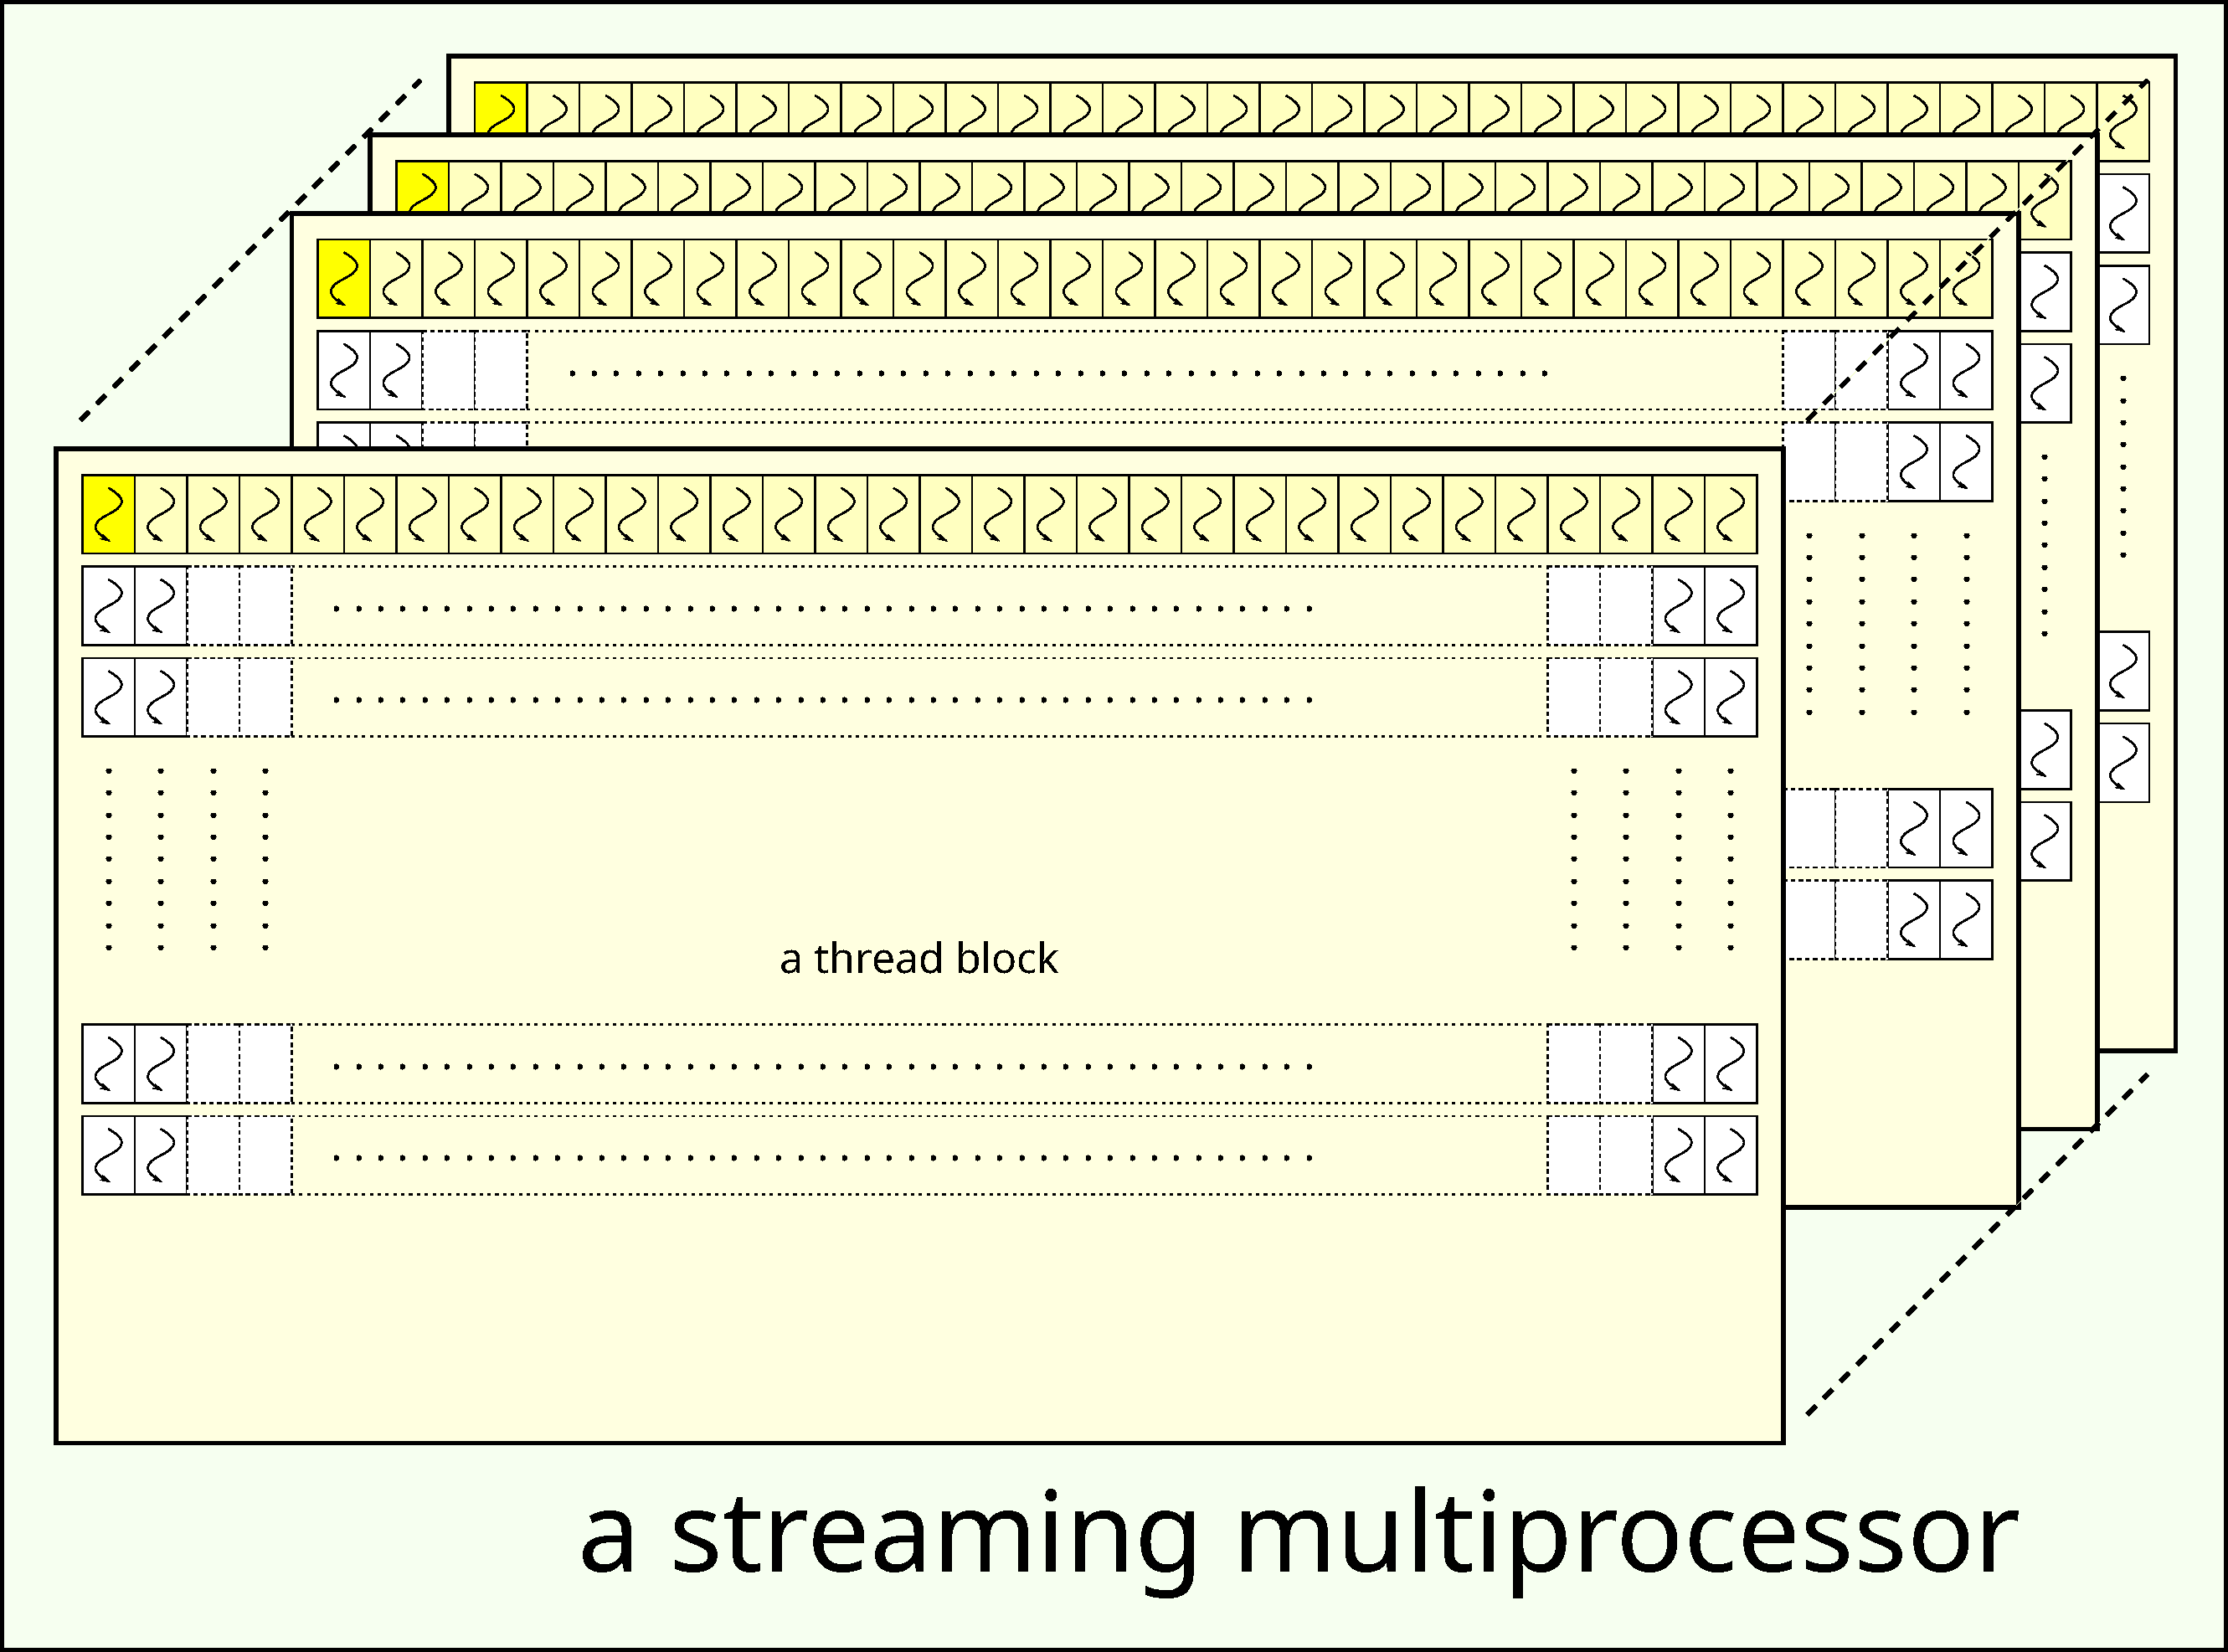
\includegraphics[width=0.9\textwidth]{out/pdf/svg/warps_blocks_4.pdf}
  \end{center}
    \end{column}
    \begin{column}{0.6\textwidth}
    two major resource constraints
    \begin{itemize}
    \item \aka{register capacity}
    \item \aka{shared memory} (covered later)
    \end{itemize}
    {\tiny
  \begin{tabular}{|l|r|r|}\hline
                & Pascal               & Volta \\\hline
  registers     & 64K $\times$ 4 bytes & 64K $\times$ 4 bytes \\
  shared memory & 64KB                 & 96KB                 \\\hline
  \end{tabular}}
  \end{column}
  \end{columns}

  \begin{itemize}
  \item registers: a thread block that has \ao{\it any} live
    ($=$ started but not finished) thread occupies
    this many registers:
    \[ \mbox{registers per thread} \times
      \mbox{the number of threads per block} \]

  \item $\Rightarrow$ the number of simultaneously live thread blocks

    \[ \leq
      \left\lfloor\frac{\mbox{register capacity}}
        {\mbox{registers per thread} \times
          \mbox{the number of threads per block}}\right\rfloor \]
  \end{itemize}
\end{frame}

\end{document}


